\pdfminorversion=4
\documentclass[aspectratio=169]{beamer}

\mode<presentation>
{
  \usetheme{default}
  \usecolortheme{default}
  \usefonttheme{default}
  \setbeamertemplate{navigation symbols}{}
  \setbeamertemplate{caption}[numbered]
  \setbeamertemplate{footline}[frame number]  % or "page number"
  \setbeamercolor{frametitle}{fg=white}
  \setbeamercolor{footline}{fg=black}
} 

\usepackage[english]{babel}
\usepackage{inputenc}
\usepackage{tikz}
\usepackage{courier}
\usepackage{array}
\usepackage{bold-extra}
\usepackage{minted}
\usepackage[thicklines]{cancel}
\usepackage{fancyvrb}

\xdefinecolor{dianablue}{rgb}{0.18,0.24,0.31}
\xdefinecolor{darkblue}{rgb}{0.1,0.1,0.7}
\xdefinecolor{darkgreen}{rgb}{0,0.5,0}
\xdefinecolor{darkgrey}{rgb}{0.35,0.35,0.35}
\xdefinecolor{darkorange}{rgb}{0.8,0.5,0}
\xdefinecolor{darkred}{rgb}{0.7,0,0}
\definecolor{darkgreen}{rgb}{0,0.6,0}
\definecolor{mauve}{rgb}{0.58,0,0.82}

\title[2023-11-15-superhistograms-irishep-topical]{SuperhistogramS \\ --- or --- \\ abstract algebra for fun and profit}
\author{Jim Pivarski}
\institute{Princeton University -- IRIS-HEP}
\date{November 15, 2023}

\usetikzlibrary{shapes.callouts}

\begin{document}

\logo{\pgfputat{\pgfxy(0.11, 7.4)}{\pgfbox[right,base]{\tikz{\filldraw[fill=dianablue, draw=none] (0 cm, 0 cm) rectangle (50 cm, 1 cm);}\mbox{\hspace{-8 cm}\includegraphics[height=1 cm]{princeton-logo-long.png}\hspace{0.1 cm}\raisebox{0.1 cm}{\includegraphics[height=0.8 cm]{iris-hep-logo-long.png}}\hspace{0.1 cm}}}}}

\begin{frame}
  \titlepage
\end{frame}

\logo{\pgfputat{\pgfxy(0.11, 7.4)}{\pgfbox[right,base]{\tikz{\filldraw[fill=dianablue, draw=none] (0 cm, 0 cm) rectangle (50 cm, 1 cm);}\mbox{\hspace{-8 cm}\includegraphics[height=1 cm]{princeton-logo.png}\hspace{0.1 cm}\raisebox{0.1 cm}{\includegraphics[height=0.8 cm]{iris-hep-logo.png}}\hspace{0.1 cm}}}}}

% Uncomment these lines for an automatically generated outline.
%\begin{frame}{Outline}
%  \tableofcontents
%\end{frame}

% START START START START START START START START START START START START START

\begin{frame}{Vague statement of the problem}
\Large
\vspace{0.5 cm}
\begin{columns}
\column{0.4\linewidth}
\only<1>{\textcolor{darkblue}{Long, long ago, histograms were individual objects that were managed individually.}}\only<2>{\textcolor{darkblue}{Now, histograms are more often used collectively, with thousands of histograms in a single fit.}}

\column{0.6\linewidth}
\only<1>{\hfill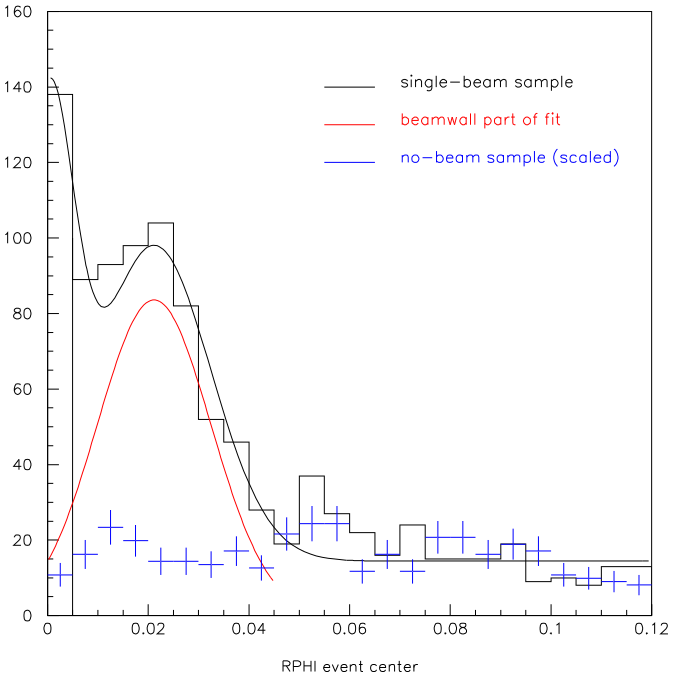
\includegraphics[width=0.8\linewidth]{old-school-histograms.pdf}}\only<2>{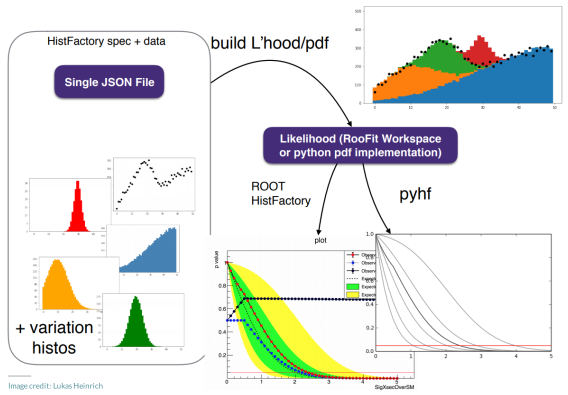
\includegraphics[width=\linewidth]{modern-histograms.pdf}}

\end{columns}
\end{frame}

\begin{frame}{Vague statement of the problem}
\vspace{0.5 cm}
\Large
\textcolor{darkblue}{A ``superhistogram'' is a large collection of histograms that are meant to be interpreted together.}
\end{frame}

\begin{frame}{Vague statement of the problem}
\vspace{0.5 cm}
\large

\textcolor{darkblue}{Representing a superhistogram with a directory of ordinary histograms is}

\vspace{0.5 cm}
\begin{itemize}\setlength{\itemsep}{0.5 cm}
\item \textcolor{darkblue}{wasteful} because much of the same metadata is copied in memory or on disk, and many small buffers of bin contents is less efficient than one big buffer.

\item \textcolor{darkblue}{inconvenient} because the object with a common meaning has to be managed as individual objects without an explicit connection. (Usually, they're linked with naming conventions.)
\end{itemize}
\end{frame}

\begin{frame}{Vague statement of the problem}
\vspace{0.5 cm}
\Large
\textcolor{darkblue}{Boost::Histogram provides a generic way to create an $n$-dimensional space with regular, variable, and categorical axes.}

\vspace{0.5 cm}
\begin{columns}
\column{0.6\linewidth}
\includegraphics[width=\linewidth]{histogram_design.png}

\column{0.4\linewidth}
\includegraphics[width=\linewidth]{axis_regular.png}

\vspace{0.35 cm}
\includegraphics[width=\linewidth]{axis_variable.png}

\vspace{0.35 cm}
\includegraphics[width=\linewidth]{axis_category.png}
\end{columns}
\end{frame}

\begin{frame}{Vague statement of the problem}
\vspace{0.5 cm}
\Large

\textcolor{darkblue}{But a Boost::Histogram is still a single histogram:}

\vspace{0.25 cm}
\begin{itemize}
\item $n$ axes form an $n$-dimensional space,
\item each scalar \mintinline{python}{fill} operation increments {\it one} bin in that space.
\end{itemize}

\vspace{0.75 cm}
\begin{uncoverenv}<2->
\textcolor{darkblue}{A superhistogram has multiple sources, channels, and systematics.}

\vspace{0.25 cm}
\begin{itemize}
\item Not all histograms in the collection have the same number of bins or the same dimensions.
\item One \mintinline{python}{fill} of the superhistogram would increment every histogram in the collection.
\end{itemize}
\end{uncoverenv}
\end{frame}

\begin{frame}[fragile]{Something like this}
\vspace{0.15 cm}
\small
\begin{minted}{python}
h = SuperHist(SuperHist(
        SuperHist(
            Hist.Reg(100, 0, 30, name="syst-up"),
            Hist.Reg(100, 0, 30, name="nominal"),
            Hist.Reg(100, 0, 30, name="syst-down"),
            name="pt",
        ),
        SuperHist(
            Hist.Reg(100, -5, 5, name="syst-up"),
            Hist.Reg(100, -5, 5, name="nominal"),
            Hist.Reg(100, -5, 5, name="syst-down"),
            name="eta",
        ),
        name="data",
    ),
    ...,   # similarly for name="mc"
)
h.fill(pandas_dataframe)   # one row is a scalar fill operation
\end{minted}
\end{frame}

\begin{frame}{So far, this is looking like Histogrammar}
\vspace{0.08 cm}
\begin{center}
\includegraphics[width=0.9\linewidth]{histogrammar-website.png}
\end{center}
\end{frame}

\begin{frame}{R.I.P. Histogrammar}
\vspace{0.5 cm}
\Large
\textcolor{darkblue}{Histogrammar was too loose: it described a {\it tree} of nested binnings (unlike Boost::Histogram's {\it sequence}), and then there was no connection among the branches of the tree.}

\vspace{1 cm}
\uncover<2->{\textcolor{darkblue}{We need a relationship that restricts the superhistogram to a useful subset of all possible trees.}}
\end{frame}

\begin{frame}{Abstract algebra for fun (profit comes later)}





\end{frame}


\end{document}
